% ======================================================================================================================
%                                                                 
% Title: Extensions
% Author: Jan JOHANNES, Ensai, Rue Blaise Pascal - BP 37203, 35172 Bruz Cedex, France
% Email: jan.johannes@ensai.fr
% Date: %%ts latex start%%[2016-05-20 Fri 03:26]%%ts latex end%%
% Main-TeX-File: 2015-01-Paris-Vortrag in der form "Name"
%
% ======================================================================================================================
\subsection{Data-driven shrinked projection estimator}
% --------------------------------------------------------------------
% <<Extensions-F1>>
% --------------------------------------------------------------------
\againframe<2>{Diff}
% --------------------------------------------------------------------
% <<Extensions-F2>>
% --------------------------------------------------------------------
\bframeVL{1-3}{3}
  \frametitle{Data-driven shrinked projection estimator}
\begin{overlayarea}{\textwidth}{\textheight}
Consider weights
\begin{equation*}
w_{\Di}^{\ObSo}:=\frac{\exp\bigg(-\frac{1}{2\ObSoNoL}\big\{-\normV{(Y/\Ev)^{\Di}}^2+3C_{\Ev}\ObSoNoL\Di\oEvs\big\}\bigg)}{\sum_{k=1}^{\DiMa}\exp\bigg(-\frac{1}{2\ObSoNoL}\big\{-\normV{(Y/\Ev)^{k}}^2+3C_{\Ev}\ObSoNoL k\oEvs[k]\big\}\bigg)}
\end{equation*}
\invisible<0>{where  % $\normV{\theta}^2_{\ObSoNoL\Evs}:=\sum_{j\geq1}(\ObSoNoL\Evs_{j})^{-1}(\theta_j)^2$
  % and
  $(Y/\Ev)^k:=(Y_j/\Ev_j\Ind{1\leq j\leq k})_{j\in\Nz}$ for $k\in\Nz$.}\\[4ex]
\invisible<-1>{The data-driven shrinked projection estimator  $\hSo=\suite{\hSo}$ given by
  \begin{equation*}
    \hSo_j = \big(1-\sum_{k=1}^{j-1}w_{\Di}^{\ObSo}\big)\times\frac{Y_j}{\Ev_j}\times\Ind{1\leq j\leq \DiMa}.
  \end{equation*}}
\\[1ex]
\invisible<-2>{{\dg Open question:}  oracle/minimax optimality up to a constant?}
\end{overlayarea}
\end{frame}
\subsection{Selfinformative Bayes limit}
% --------------------------------------------------------------------
% <<Extensions-F2>>
% --------------------------------------------------------------------
\bframeVL{1-5}{5}
  \frametitle{Selfinformative Bayes limit}
\begin{overlayarea}{\textwidth}{\textheight}
{\db Iterative procedure}:\\[1ex]
given  prior $P_{\RvSo}$ and likelihood $P_{\ObSo|\RvSo}$  consider
\begin{ListeN}[\setListeV{1ex}{1.5ex}{5ex}{0ex}\renewcommand{\theListeN}{\arabic{ListeN}.}]
\item<2-> $(\ObSo_1,\RvSo_1)$ with $P_{\RvSo_1}:=P_{\RvSo}$ and
  $P_{\ObSo_1|\RvSo_1}:=P_{\ObSo|\RvSo}$\\[1ex]
$\hookrightarrow$ posterior  distribution $P_{\RvSo_1|\ObSo_1}$
\item<3-> $(\ObSo_2,\RvSo_2)$ with $P_{\RvSo_2}:=P_{\RvSo_1|\ObSo_1}$ and
  $P_{\ObSo_2|\RvSo_2}:=P_{\ObSo|\RvSo}$\\[1ex]
$\hookrightarrow$ posterior distribution $P_{\RvSo_2|\ObSo_2}$
\item<4-> $(\ObSo_3,\RvSo_3)$ with $P_{\RvSo_3}:=P_{\RvSo_2|\ObSo_2}$ and
  $P_{\ObSo_3|\RvSo_3}:=P_{\ObSo|\RvSo}$\\[1ex]
$\hookrightarrow$ posterior distribution $P_{\RvSo_3|\ObSo_3}$
\item<5->[{\dgrau$\vdots$}] 
\end{ListeN}
\invisible<-4>{{\dgrau$\eta$-th} iteratively determined
  $P_{\RvSo_\eta|\ObSo_\eta}$ depending on
  $P_{\RvSo_1|\ObSo_1},\dotsc,P_{\RvSo_{\eta-1}|\ObSo_{\eta-1}}$.}%\\[2ex]
\end{overlayarea}
\end{frame}
% --------------------------------------------------------------------
% <<Extensions-F2>>
% --------------------------------------------------------------------
\bframeVL{1-3}{3}
\frametitle{Selfinformative Bayes limit}
\begin{overlayarea}{\textwidth}{\textheight}
Consider for $\eta\in\Nz$ a determination $P_{\RvSo_\eta|\ObSo_\eta}$
of the {\db$\eta$-th posterior} and the {\db Bayes estimate $\htheta_\eta:=\Ex[\RvSo_\eta|\ObSo_\eta]$}.\\[2ex]
\mywsboxinvisible{-1}{\mbox{The limit  $\db\lim\limits_{\eta\to\infty}\htheta_\eta$  (if it exists) is
    called {\db selfinformartive Bayes limit}.}}%\hfill\\[0ex]
\invisible<-2>{\centerline{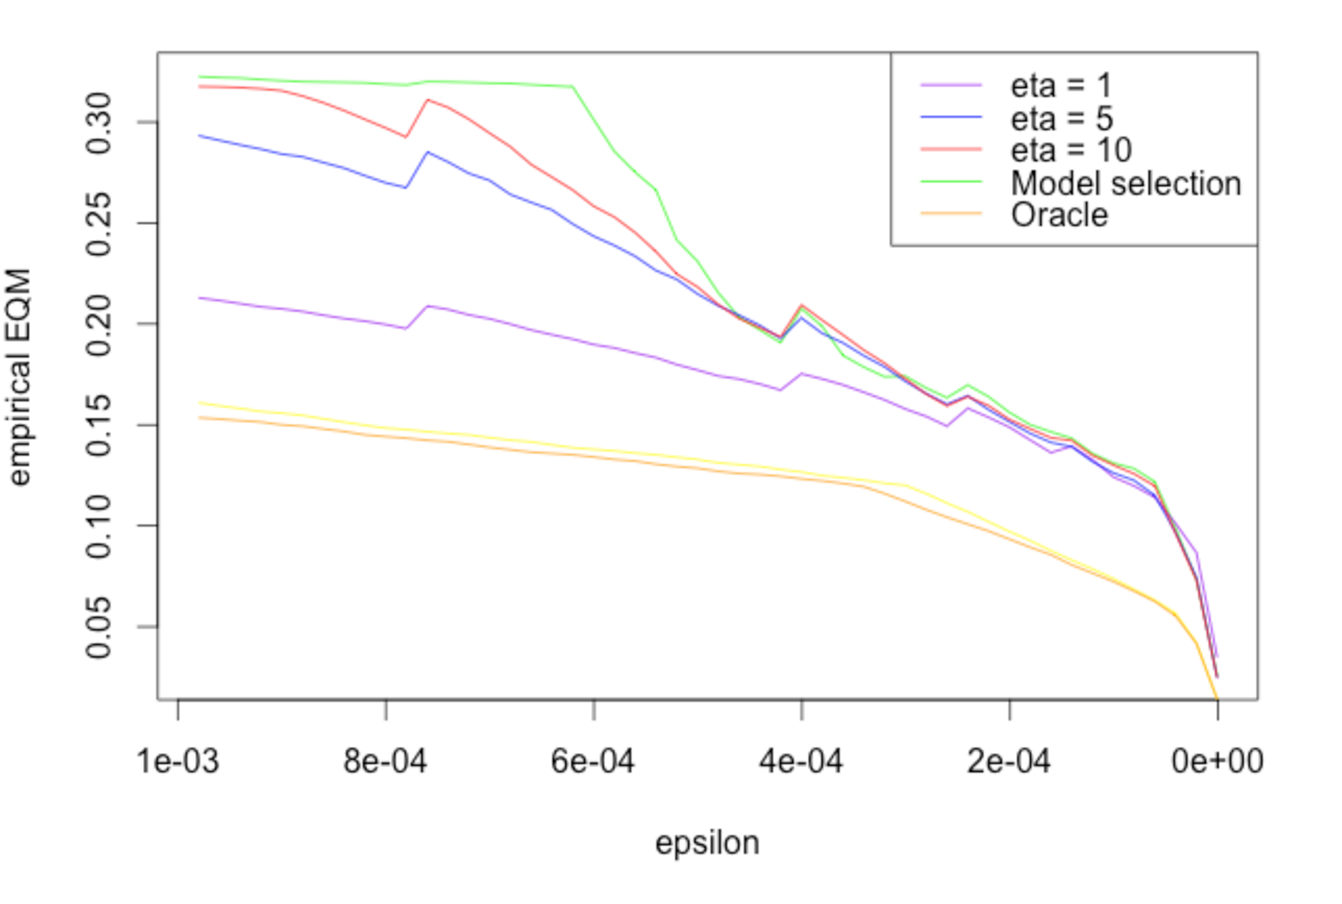
\includegraphics[width=.75\textwidth]{./Images/IterativeBayes.pdf}}}
\end{overlayarea}
\end{frame}
\subsection{Application: deconvolution}
% --------------------------------------------------------------------
% <<Extensions-F3>>
% --------------------------------------------------------------------
\bframeVL{1-8}{8}%2
\frametitle{\rudicolor Migrating birds’ navigation abilities}
\framesubtitle{\rudicolor Circular data}
\hspace{3cm}
\includegraphics<1>{./Images/pic.1}
\includegraphics<2-3>{./Images/pic.2}
\includegraphics<4>{./Images/pic.3}
\includegraphics<5>{./Images/pic.4}
\includegraphics<6>{./Images/pic.5}
\includegraphics<7>{./Images/pic.6}
\includegraphics<8->{./Images/pic.7}

\vspace{-3.5cm}
\onslide+<3-6>{\ \hspace{5.8cm}
\includegraphics[scale=.1]{./Images/tux.png}}

\vspace{3cm}
\begin{rudiListeT}[\setListe{.5ex}{.5ex}{5ex}]
\item<4-> Object of interest: density of a circular
  r.v. $\db X\sim\xdf$;
\item<5-> Noise: circular r.v. $\db\decNo\sim\edf$;
\item<6-> Observation: noisy circular r.v. $\db Y=X+\decNo\sim\ydf$
\end{rudiListeT}
\end{frame}
% --------------------------------------------------------------------
% <<Extensions-F4>>
% --------------------------------------------------------------------
\bframeVL{1-10}{2,5,10}%
\centerline{\begin{tabular}{@{}cc@{}}
Circular density  & \dwonly{1}Circular convolution\\[2ex]
\includegraphics<1-3>[scale=.6]{./Images/wow0b.pdf}%
\includegraphics<4>[scale=.6]{./Images/wow1b.pdf}%
\includegraphics<5>[scale=.6]{./Images/wow2b.pdf}%
\includegraphics<6>[scale=.6]{./Images/wow3b.pdf}%
\includegraphics<7>[scale=.6]{./Images/wow4b.pdf}%
\includegraphics<8>[scale=.6]{./Images/wow5b.pdf}%
\includegraphics<9>[scale=.6]{./Images/wow6b.pdf}%
\includegraphics<10>[scale=.6]{./Images/wow7b.pdf}%
\includegraphics<11>[scale=.6]{./Images/wow8b.pdf}%
\includegraphics<12>[scale=.6]{./Images/wow9b.pdf}%
&%
\invisible<1>{\includegraphics<1-2>[scale=.6]{./Images/wow0.pdf}}%
\includegraphics<3-4>[scale=.6]{./Images/wow1.pdf}%
\includegraphics<5>[scale=.6]{./Images/wow2.pdf}%
\includegraphics<6>[scale=.6]{./Images/wow3.pdf}%
\includegraphics<7>[scale=.6]{./Images/wow4.pdf}%
\includegraphics<8>[scale=.6]{./Images/wow5.pdf}%
\includegraphics<9>[scale=.6]{./Images/wow6.pdf}%
\includegraphics<10>[scale=.6]{./Images/wow7.pdf}%
\includegraphics<11>[scale=.6]{./Images/wow8.pdf}%
\includegraphics<12>[scale=.6]{./Images/wow9.pdf}%
\\$\decSo$ &  \dwonly{1}$\ydf=\edf\star\decSo$
\end{tabular}}
\end{frame}
% --------------------------------------------------------------------
% <<Extensions-F5>>
% --------------------------------------------------------------------
\bframeVL{1-10}{10}
\frametitle{Circular deconvolution}%
\hfill\\[-5ex]
\begin{overlayarea}{\textwidth}{.4\textheight}%
\invisible<1>{\only<1-6>{Representation:}%
\only<7-9>{Let $k\in\Nz$. }%
\only<7>{{\db Projection}:}%
\only<8-9>{{\dbonly{8}Estimator} under {\invisible<8>{\dbonly{9}un}{\dbonly{9}known}} error density:}%
\only<10>{{\db Data-driven} estimator {\db by model selection} under unknown error density:}%
\begin{multline*}%
\only<1-6>{f_{\only<7->{\dbonly{7}k}}}%
\only<7>{f_{\only<7->{\dbonly{7}k}}:}%
\only<8-9>{\hf_k:}%
\only<10>{\hf_{\db\whk}:}%
=
\only<1-7>{\invisible<-2>{{\dbonly{3} \1+}}\sum_{\only<1-2>{j\in\Zz}\only<3->{0<\dbonly{3}|j|\only<7->{\dbonly{7}\leq k}}} \only<-5>{\dbonly{2}\fou{\xdf}_j}\only<6->{{\dbonly{6}\frac{\fou{\ydf}_j}{\fou{\edf}_j}}} \ef_j}%
\only<8>{\1+\sum_{0<|j|\leq k} \frac{\dbonly{8}\hfou{\ydf}_j}{\fou{\edf}_j} \ef_j}%
\only<9>{\1+\sum_{0<|j|\leq k} \frac{\hfou{\ydf}_j}{\dbonly{9}\hfou{\edf}_j} \ef_j {\dbonly{9}\Ind{|\hfou{\edf}_j|^2\geq 1/m}}}%
\only<10>{\1+\sum_{0<|j|\leq \db \whk} \frac{\hfou{\ydf}_j}{\dbonly{9}\hfou{\edf}_j} \ef_j {\dbonly{9}\Ind{|\hfou{\edf}_j|^2\geq 1/m}}}%
\\
\hfill
\invisible<-9>{{\db\whk}:=\argmin_{1\leq k\leq \db\widehat{K}}\big\{-\normV{\hf_k}^2 + {\db\hpen}_k\big\}}
\end{multline*}}
\end{overlayarea}
\begin{overlayarea}{\textwidth}{.62\textheight}%
\hrule\hfill\\[-.5ex]
\hfill{\dgrau\footnotesize (JJ \& Schwarz, 2013)}\\
\only<1-10>{\textbf{Notation/Recall}: $\dbonly{1} X\sim \xdf$\invisible<-3>{, $\dbonly{4}\epsilon\sim\edf$   and $\dbonly{4} Y\sim \ydf=\xdf\star\edf$}\\[1em]}%
\only<-10>{%
\begin{tabular}{l@{\hspace{1ex}}l}
\invisible<1>{Orthonormal basis:&  ${\dbonly{2} \ef_j}=\exp(-\iota 2\pi j\bullet),$\\[.7em]}%
\invisible<1>{Fourier coefficients:&  \small ${\dbonly{2}\fou{\xdf}_j}=\Ex[\ef_j(-X)],$ \invisible<-3>{${\dbonly{4}\fou{\edf}_j}=\Ex[\ef_j(-\decNo)],$ ${\dbonly{4}\fou{\ydf}_j}=\Ex[\ef_j(-Y)],$}\\[.7em]}%
\invisible<-4>{Convolution theorem:& $\dbonly{5}\ydf=\xdf\star\edf$ iff $\dbonly{5}\fou{\ydf}_j = \fou{\xdf}_j\,\fou{\edf}_j$, $\forall j\in\Zz$\\[.7em]}%
\invisible<-7>{Estimated coeff.:&  ${\dbonly{8}\hfou{\ydf}_j} := \frac{1}{n}\sum_{k=1}^n\ef_j(-Y_k)$, \invisible<-8>{${\dbonly{9}\hfou{\edf}_j} := \frac{1}{m}\sum_{k=1}^m\ef_j(-\decNo_k)$}\\[.7em]}
\end{tabular}}
\end{overlayarea}
\end{frame}
% --------------------------------------------------------------------
% <<Extensions-F6>>
% --------------------------------------------------------------------
\bframeVL{1-3}{3}
  \frametitle{Data-driven shrinked deconvolution estimator}
\begin{overlayarea}{\textwidth}{\textheight}
Consider weights
\begin{equation*}
{\db w_{\Di}^Y}:=\frac{\exp\bigg(-n\big\{-\normV{\hfou{\ydf}^{\Di}}^2+c\Di/n\big\}\bigg)}{\sum_{k=1}^{\DiMa}\exp\bigg(-n\big\{-\normV{\hfou{\ydf}^{k}}^2+ck/n\big\}\bigg)}
\end{equation*}
\invisible<0>{where  % $\normV{\theta}^2_{\ObSoNoL\Evs}:=\sum_{j\geq1}(\ObSoNoL\Evs_{j})^{-1}(\theta_j)^2$
  % and
  $\hfou{\ydf}^k:=(\hfou{\ydf}_j\Ind{1\leq j\leq k})_{j\in\Nz}$ for $k\in\Nz$.}\\[4ex]
\invisible<-1>{The data-driven shrinked deconvolution estimator  is given by
  \begin{equation*}
    {\hf:}%
=
\1+\sum_{0<|j|\leq G_n} {\db\big(1-\sum_{\Di=1}^{j-1}w_{\Di}^Y\big) }\frac{\hfou{\ydf}_j}{\dbonly{9}\hfou{\edf}_j} \ef_j {\dbonly{9}\Ind{|\hfou{\edf}_j|^2\geq 1/m}}.
  \end{equation*}}
\\[1ex]
\invisible<-2>{{\dg Open question:}  oracle/minimax optimality up to a constant?}
\end{overlayarea}
\end{frame}
% \bframeVL{1-2}{2}
% \frametitle{Data-driven shrinked deconvolution estimator:}%
% \hfill\\[-5ex]
% \begin{overlayarea}{\textwidth}{.6\textheight}%
% \begin{multline*}%
% {\hf:}%
% =
% \1+\sum_{0<|j|\leq G_n} {\db\big(1-\sum_{\Di=1}^{j-1}w_{\Di}^Y\big) }\frac{\hfou{\ydf}_j}{\dbonly{9}\hfou{\edf}_j} \ef_j {\dbonly{9}\Ind{|\hfou{\edf}_j|^2\geq 1/m}}%
% \\[2ex]
% \hfill
% {\db w_{\Di}^Y}:=\frac{\exp\bigg(-n\big\{-\normV{\hfou{\ydf}^{\Di}}^2+c\Di/n\big\}\bigg)}{\sum_{k=1}^{\DiMa}\exp\bigg(-n\big\{-\normV{\hfou{\ydf}^{k}}^2+ck/n\big\}\bigg)}
% \end{multline*}
% \end{overlayarea}
% \begin{overlayarea}{\textwidth}{.62\textheight}%
% %\hrule\hfill\\[1ex]
% \invisible<1>{{\dg Open question:}  oracle/minimax optimality up to a constant?}
% \end{overlayarea}
% \end{frame}


%%% Local Variables:
%%% mode: latex
%%% TeX-master: "_2016-05-LLN-Vortrag"
%%% End:
